%!TEX root = ../paper.tex

\subsubsection{Data Type}
\label{sec:datatypes}

Based on our statistical models (later reported in Section \ref{sec:regression}), we observed that the largest effect on participants' VURs stemmed from the type of data being shared; data recipient and device type had weaker impacts on overall VURs. The most and least concerning data types are listed in Table \ref{top10-table}, and the full list can be seen in Table \ref{full-vur-table} in Appendix \ref{sec:concerns-appendix}. 

Participants were most concerned about photos and videos, especially if they contained embarrassing content, nudity, or financial information. As seen in Table \ref{top10-table}, photos and videos accounted for five of the top ten concerns, and are almost unanimously considered to be concerning. Information that could be used to impersonate someone (e.g., usernames/passwords for websites), or photos of someone at home, were also among the most concerning data types. 

Participants were least concerned about data that could be collected through observations of public behavior, such as demographics (e.g., age, gender, language) or information available to advertisers (e.g., TV shows watched, music on device). As seen in Table \ref{top10-table}, participants' responses had a greater amount of variance.  This greater variance and overall decreased concern may be because of uncertainty with how the data would be used, or because the financial, social, or physical consequences would be less immediate.

Although certain data is considered unanimously upsetting to have shared, it is interesting to note that no data was considered unanimously non-upsetting to have shared, nor were there any data types that evoked strong disagreement between participants (i.e., bimodal). Generally, the average concern magnitude was inversely correlated with the standard deviation, which suggests the presence of ceiling effects for the most concerning data types. For the complete ranked list of data types in this study, see Appendix \ref{sec:data-appendix}.

\begin{table*}[t]
\begin{center}
\small
\begin{tabular}{| r | l | r | r |c |}
\hline
Rank & Data & VUR & $\sigma$ & Distribution \\
\hline
1 & video of you unclothed & 95.97\% & 0.31 & 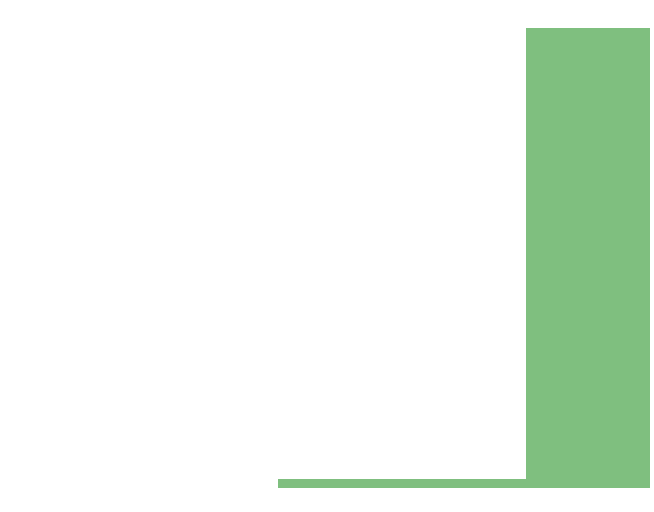
\includegraphics[width = 2cm, height = 0.5cm]{tex-inputs/data10/tookavideoofyouunclothedcombined} \\
2 & bank account information & 95.91\% & 0.35 & 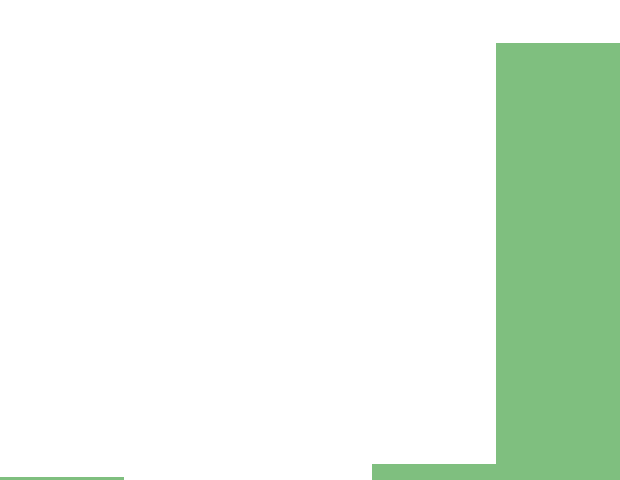
\includegraphics[width = 2cm, height = 0.5cm]{tex-inputs/data10/learnedyourbankaccountinformationcombined}  \\
3 & social security number & 94.84\% & 0.26 & 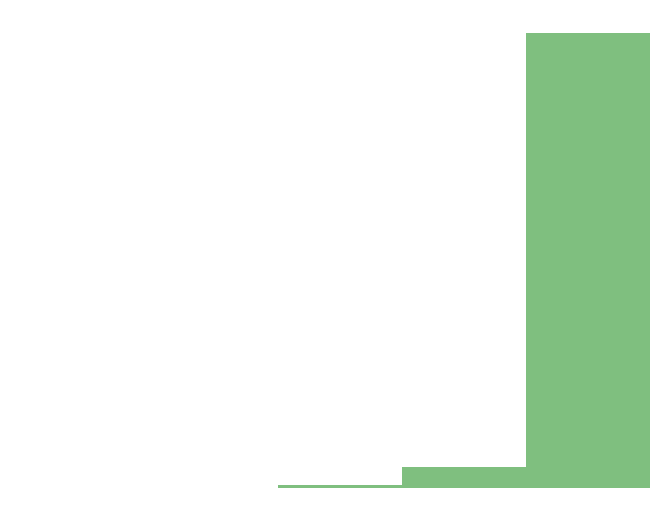
\includegraphics[width = 2cm, height = 0.5cm]{tex-inputs/data10/learnedyoursocialsecuritynumbercombined}\\
4 & video entering in a PIN at an ATM & 92.67\% & 0.47 & 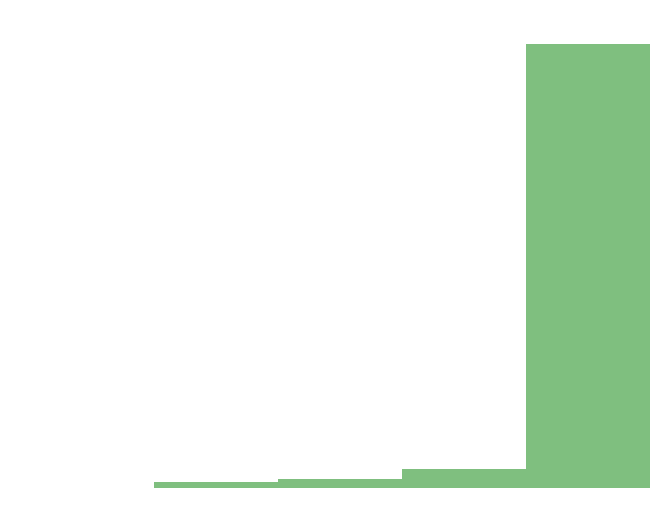
\includegraphics[width = 2cm, height = 0.5cm]{tex-inputs/data10/tookavideoofyouenteringinyourPINatanATMcombined}\\
5 & photo of you unclothed & 92.59\% & 0.46 & 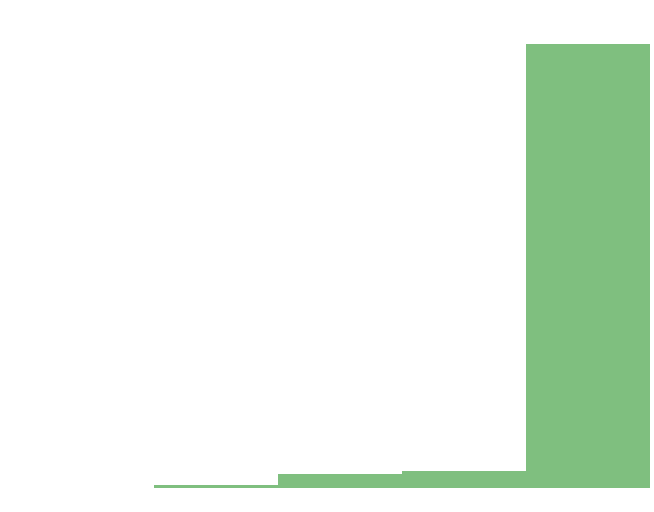
\includegraphics[width = 2cm, height = 0.5cm]{tex-inputs/data10/tookaphotoofyouunclothedcombined}\\
6 & photo of you that is very embarrassing & 91.39\% & 0.55 & 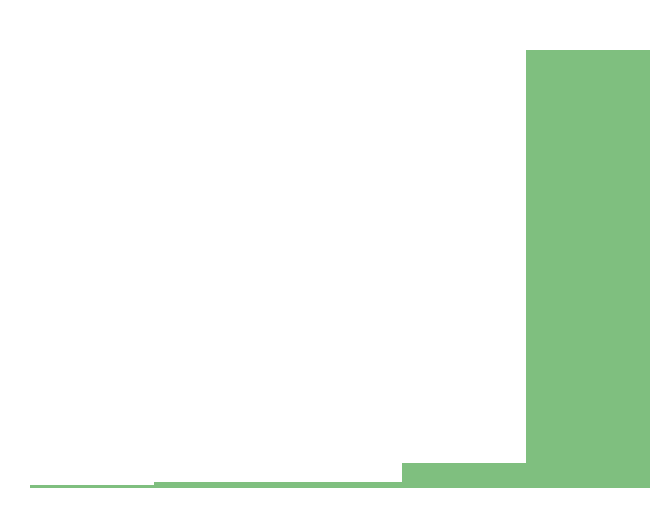
\includegraphics[width = 2cm, height = 0.5cm]{tex-inputs/data10/tookanincriminatingphotoofyoudoingsomethingembarrassingcombined}\\
7 & username and password for websites & 89.55\% & 0.62 & 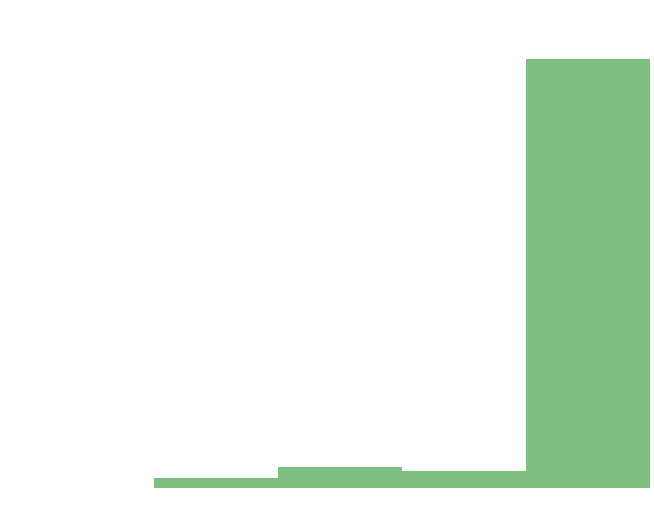
\includegraphics[width = 2cm, height = 0.5cm]{tex-inputs/data10/learnedyourusernameandpasswordforwebsitescombined}\\
8 & credit card information & 88.98\% & 0.56 & 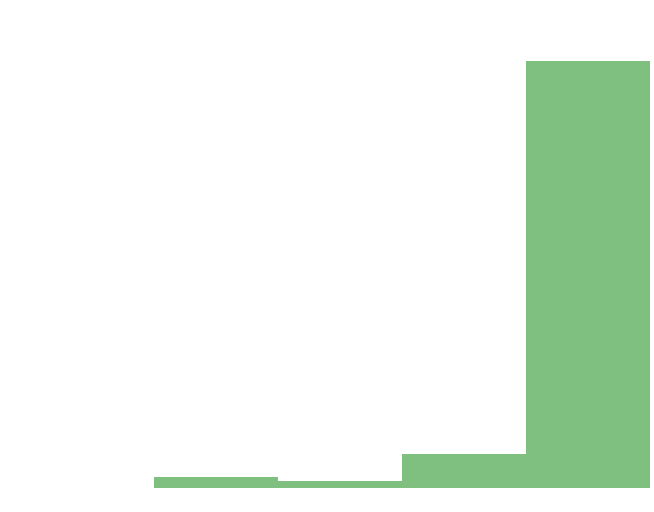
\includegraphics[width = 2cm, height = 0.5cm]{tex-inputs/data10/learnedyourcreditcardinformationcombined}\\
9 & video of you that is very embarrassing & 88.41\% & 0.53 & 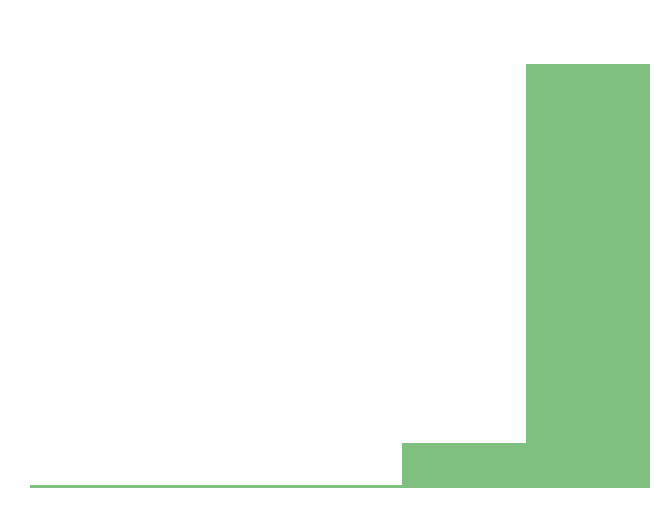
\includegraphics[width = 2cm, height = 0.5cm]{tex-inputs/data10/tookanincriminatingvideoofyoudoingsomethingembarrassingcombined}\\
10 & photo of you at home & 87.50\% & 0.60 & 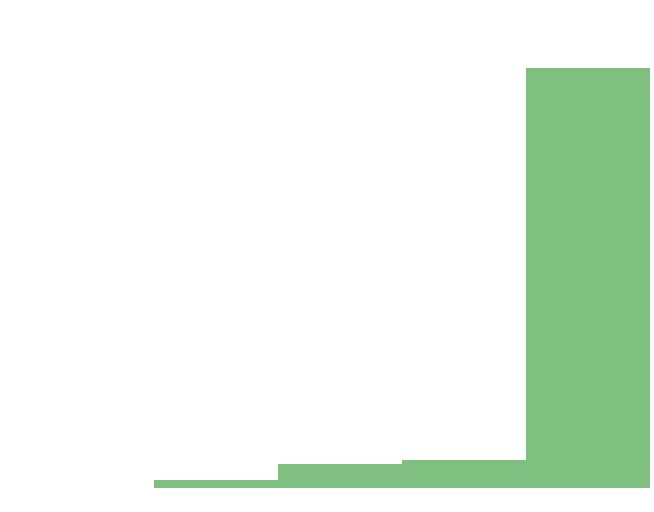
\includegraphics[width = 2cm, height = 0.5cm]{tex-inputs/data10/tookphotosofyou(withaninward-facingcamera)athomecombined}\\
 & \vdots & & & \\
64 & eye patterns (for eye tracking) & 40.51\%& 1.27 & 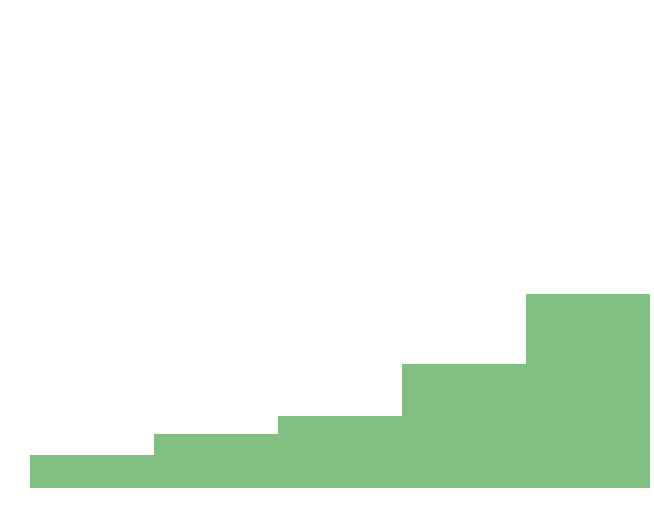
\includegraphics[width = 2cm, height = 0.5cm]{tex-inputs/data10/scannedyoureyetolearnyoureyepatterns(foreyetracking)combined} \\
65 & exercise patterns  & 38.66\% & 1.26 & 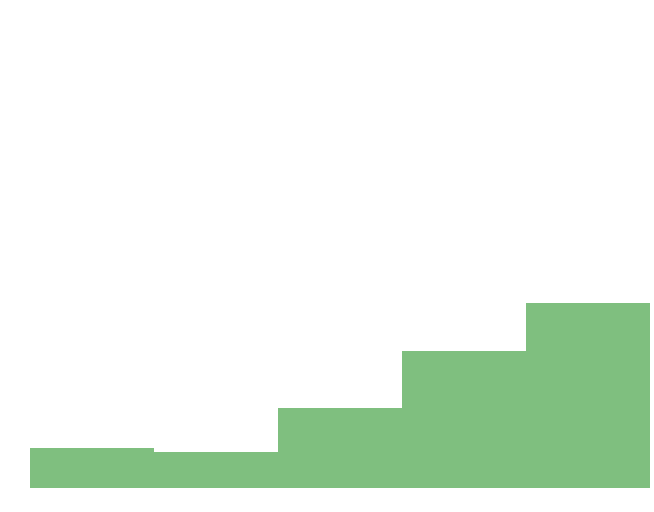
\includegraphics[width = 2cm, height = 0.5cm]{tex-inputs/data10/learnedwhenhowandhowmuchyouexercisecombined}\\
66 & when you are happy or having fun  & 34.75\% & 1.27 & 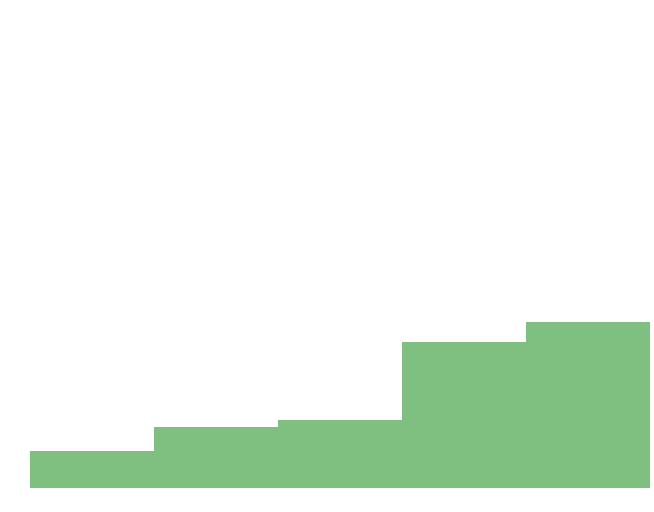
\includegraphics[width = 2cm, height = 0.5cm]{tex-inputs/data10/learnedwhenyouwerehappyorhavingfuncombined}\\
67 & television shows watched & 30.20\% & 1.40 & 
\includegraphics[width = 2cm, height = 0.5cm]{tex-inputs/data10/learnedwhattelevisionshowsyouwatchcombined}\\
68 & when you are busy or interruptible  & 29.50\% & 1.26 & 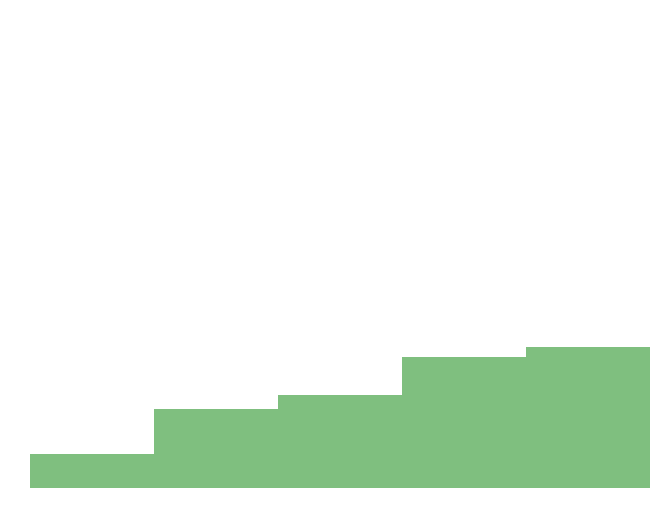
\includegraphics[width = 2cm, height = 0.5cm]{tex-inputs/data10/learnedwhenyouarebusyorinterruptiblecombined}\\
69 & music on device  & 28.06\% & 1.43 & 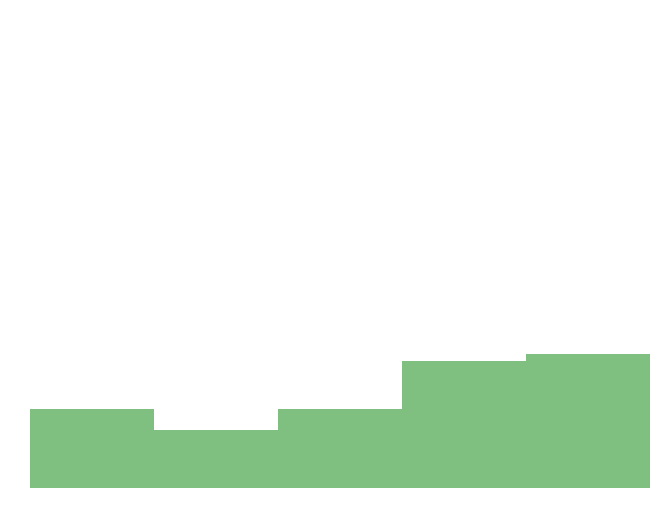
\includegraphics[width = 2cm, height = 0.5cm]{tex-inputs/data10/copiedanduploadedmusicfromyourdevicecombined}\\
70 & your heart rate & 27.50\% & 1.40 & 
\includegraphics[width = 2cm, height = 0.5cm]{tex-inputs/data10/learnedyourheartratecombined} \\
71 & age & 24.29\% & 1.43 & 
\includegraphics[width = 2cm, height = 0.5cm]{tex-inputs/data10/learnedyouragecombined}\\
72 & language spoken & 15.86\% & 1.49 & 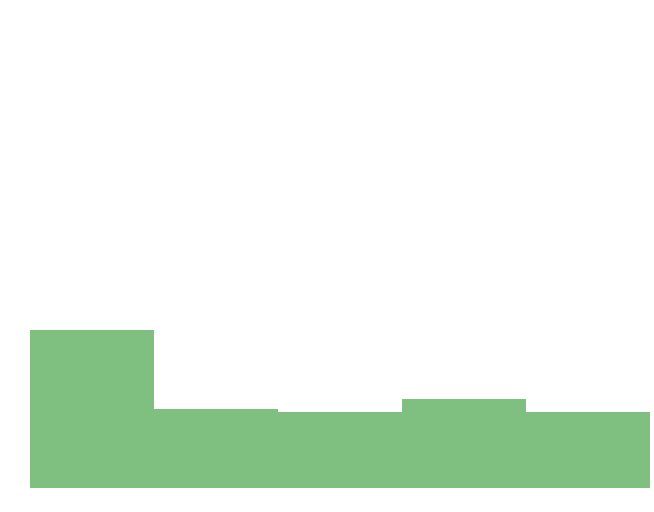
\includegraphics[width = 2cm, height = 0.5cm]{tex-inputs/data10/learnedthelanguageyouwerespeakingcombined}\\
73 & gender & 15.00\% & 1.45 & 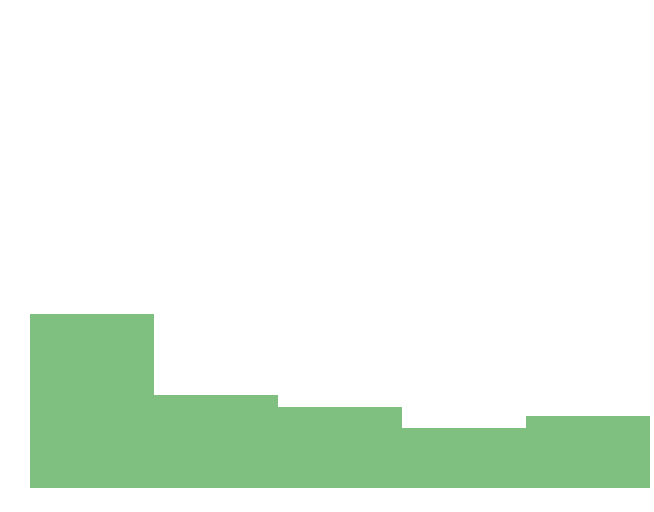
\includegraphics[width = 2cm, height = 0.5cm]{tex-inputs/data10/learnedyourgendercombined}\\ 
\hline
\end{tabular}
\caption{The 10 most and least upsetting data types, across all recipients. For the complete list of all data types across all recipients, see Appendix \ref{sec:data-appendix}.}
\label{top10-table}
\end{center}
\end{table*}


%A statistical analysis regarding the significance and confidence of <data> types with respect to all 72 was not performed due to the space constraints of the paper. We do consider all <data> categories in our statistical model, which provides an analysis of what factors had contributed to the perceived severity of a particular situation. 









